% Source: https://tex.stackexchange.com/a/639280
\documentclass[tikz]{standalone}
    
\usepackage{tzplot}

\begin{document}

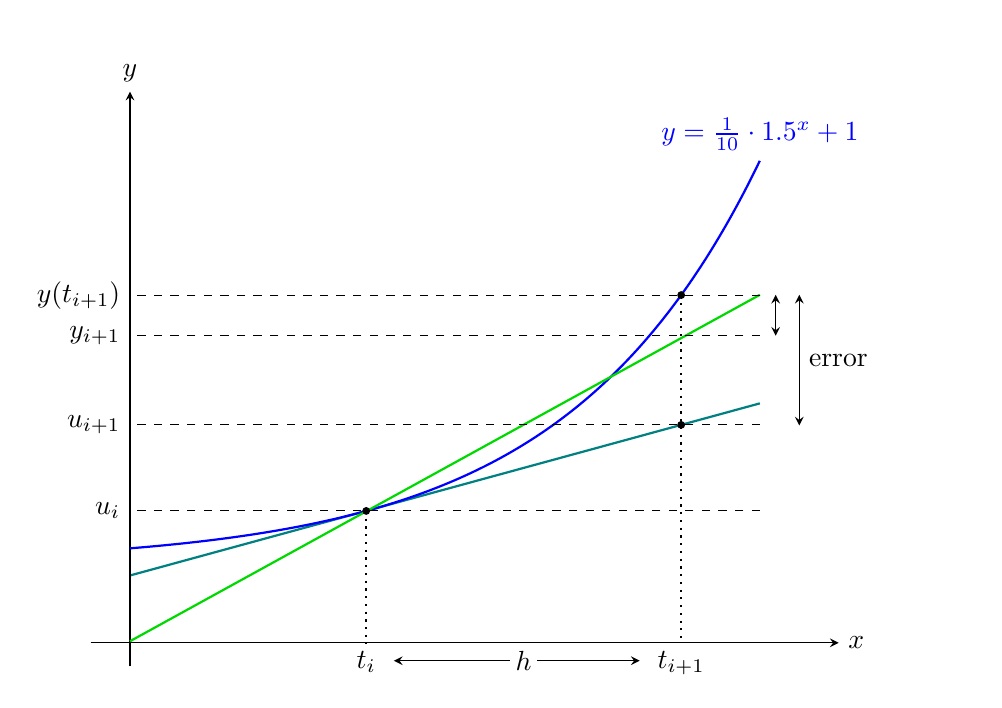
\begin{tikzpicture}
% \tzhelplines(9,7)
\tzaxes(-.5,-.3)(9,7){$x$}{$y$}
\def\Fx{.2*1.5^\x+1}
\tzfn[thick,blue]\Fx[0:8]{$y=\frac1{10}\cdot1.5^x+1$}[a]
\tztangentat[green!50!blue,thick]"tan"{Fx}{3}[0:8]
% \draw[domain=0:8, variable=\x, green!85!black, thick] plot ({\x}, {0.275*(\x-3)+1.67});
\draw[domain=0:8, variable=\x, green!85!black, thick] plot ({\x}, {0.55*(\x-3)+1.67});
% \draw[domain=0:8, variable=\x, red, thick] plot ({\x}, {1.4*(\x-7)+4.42});
% intersections
\tzvXpointat*{Fx}{7}(A)
\tzvXpointat*{tan}{7}(B)
\tzvXpointat*{Fx}{3}(C)
% projections on x-axis
\tzprojsx[thick](C){$t_i$}(A){$t_{i+1}$}; % version 2
% horizontal dashed lines
\tzhfn[dashed](A)[8:0]{$y(t_{i+1})$}[l]
\tzhfn[dashed](B)[8:0]{$u_{i+1}$}[l]
\tzhfn[dashed](C)[8:0]{$u_i$}[l]
\tzhfn[dashed](6,3.9)[8:0]{\(y_{i+1}\)}[l]
% labels
\tzline[<->]<1.2,0>(7.3,4.42){error}[r](7.3,2.76)
\tzline[<->]<1.2,0>(7,4.42)[r](7,3.9)
% \tzline+[->](3,3.5){Tangent line}[at start,a](2.5,-1)
% \tznode(6,3.5){$f(t_i,u_i)$}[l]
\tzline[<->,tzshorten={1em}{1.5em}]
       (C|-{0,-1.5ex}){$h$}[inner sep=2pt,centered,fill=white]
       (A|-{0,-1.5ex})
\end{tikzpicture}

\end{document}